\documentclass[11pt]{article}
\usepackage{makeidx}
\usepackage{multirow}
\usepackage{multicol}
\usepackage[dvipsnames,svgnames,table]{xcolor}
\usepackage{graphicx}
\usepackage{epstopdf}
\usepackage{ulem}
\usepackage{hyperref}
\usepackage{amsmath}
\usepackage{amssymb}
\author{Livio Ferrante}
\title{}
\usepackage[paperwidth=595pt,paperheight=841pt,top=70pt,right=56pt,bottom=56pt,left=56pt]{geometry}

\makeatletter
	\newenvironment{indentation}[3]%
	{\par\setlength{\parindent}{#3}
	\setlength{\leftmargin}{#1}       \setlength{\rightmargin}{#2}%
	\advance\linewidth -\leftmargin       \advance\linewidth -\rightmargin%
	\advance\@totalleftmargin\leftmargin  \@setpar{{\@@par}}%
	\parshape 1\@totalleftmargin \linewidth\ignorespaces}{\par}%
\makeatother 

% new LaTeX commands


\begin{document}


{\raggedright
\textbf{PhD student Livio Ferrante}
}

{\raggedright
\textbf{Effective Programming Practices for Health Economists\\
A short report on my {\small
hypothetical final project}}}\\
{\raggedright
I created a private repository in my educational account on Github. The URL is \\
 https://github.com/livioferrante/my-final-project
}

{\raggedright
I cloned the template that you provided the last day of the course on my repository. I hypothetically use Python, otherwise I should switch on branch to specify the language that I'll use most (e.g. stata, r, matlab...).
}

{\raggedright
As I showed you, Waf doesn't run in my machine, then I'm using my repository to put this report about what I would do... if Waf runs!! Therefore, I created a new branch called "report" and I'm working in it with a tex file ( \textit{git branch report}   /   \textit{git checkout report} ).
}

{\raggedright
The ratio behind the use of Waf lies in the "reproducibility". Waf is a tool, written in Python, that allows to automate the dependency tracking via a DAG structure (Directed Acyclic Graph). Replicability of results is an important issue in scientific research and is became a fundamental tool in many economic journals which nowadays are implementing strict replication policies. Moreover, it allows to avoid huge waste of time and resources as well as potential errors.
}

{\raggedright One could do all it manually by typing stuff to the console and clicking buttons. But it would be hard to track the sequence of clicks and runs one had to do to end up with the final document. So Waf is basically a long list of commands that runs everything in the right order to end up with the final document, presentation and several other things. To make it a little more convenient for the users, Waf can check different folders for the commands, so one doesn't need a huge wscript but can have several small ones located where they'd logically belong.}\\

{\raggedright
Example of a personal project:\\
}
{\raggedright
Currently, I haven't a personal project, then I imagined to implement a simple research structure which could fit with a creation of an empirical paper.
}

{\raggedright
First of all, I created the dependency graph for my project:
}

\begin{figure}[htbp] 
	\centering 
	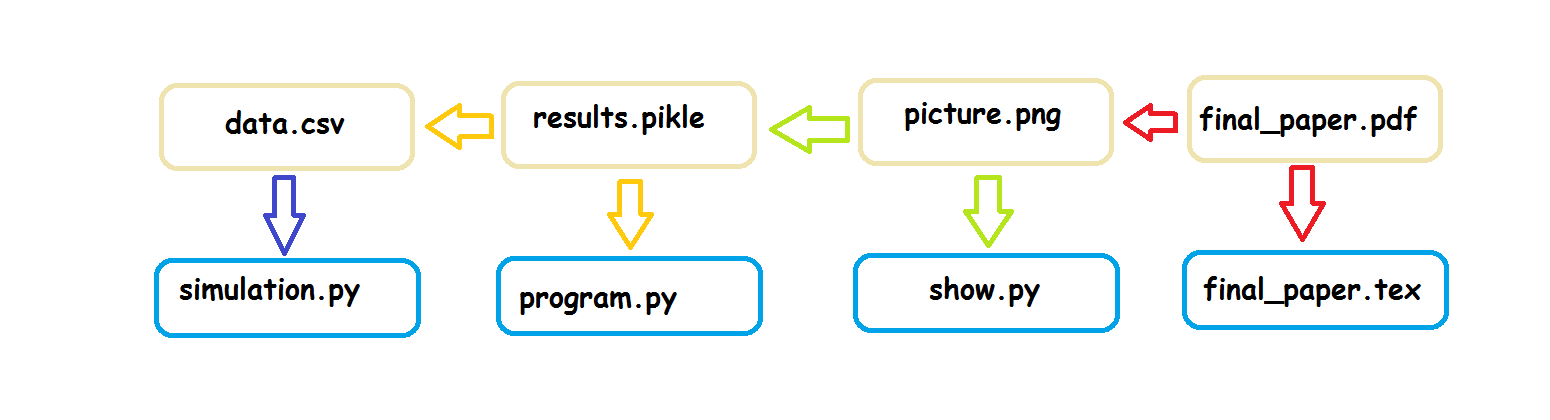
\includegraphics[scale=0.4]
	{effective.png} 
	\caption{Dependency graph} 
	\label{fig:figuraSingola} 
\end{figure}

{\raggedright
The colors of arrows distinguish the steps of the analysis: blue is used for data management, orange for the simulation, green for the visualization of a graph, red to get work in a pdf file.
Blue circled nodes represent source files; brown circled nodes represent target files generated by the code depending on source files. 
In the first run, Waf generates all the targets, whereas in the later runs Waf generates only targets for which dependencies are changed. Then Waf is very useful to gain time whenever one runs big projects. 
}

{\raggedright
Wscript files are the entry point for the instructions given to Waf. Every wscript holds build information, that are commands that run the data processing scripts,  computing scripts, plotting scripts, etc. 
Waf works recursively: it means a wscript file checks whether there are any subfolders that also contain wscripts (this is done until the "bottom of the barrel"). By specifying dependencies and targets correctly, wscripts realize what parts depend on each other and whether things could be run in parallel or have to wait for another script to be finished.
}

{\raggedright
First of all, one should set up a suitable folder structure in the source. Folder src (source) contains the structure; all stuff that is created lands in the build folder (bld). 
 

}

{\raggedright
One has to put the following command line to start the process: ~
}

{\raggedright
\textit{{\small python waf.py configure  }}
}

{\raggedright
{\small and in the main wscript file, in order to configure the correct paths:}
}

{\raggedright
\textit{{\small def build(ctx):}}
}

{\raggedright
\textit{{\small     ctx.recurse('src')}}
}

{\raggedright
{\small and inside the file src/wscript:}
}

{\raggedright
\textit{{\small def build(ctx):}}
}

{\raggedright
\textit{{\small     ctx.recurse('data\_management')}}
}

{\raggedright
\textit{{\small     ctx.recurse('analysis')}}
}

{\raggedright
\textit{{\small     ctx.recurse('final')}}
}

{\raggedright
\textit{{\small     ctx.recurse('paper')}}
}

{\raggedright
{\small Now, in order to establish the dependency structure, one has to compile the contents of wscript files.
}
}

{\raggedright
{\small 
For the first dependency of the project, one has to put inside the file:}
}

{\raggedright
\textit{{\small src/data\_management/wscritp}}
}

{\raggedright
{\small the code:}
}

{\raggedright
\textit{{\small \#! python}}
}

{\raggedright
\textit{{\small def build(ctx):}}
}

{\raggedright
\textit{{\small     ctx(}}
}

{\raggedright
\textit{{\small         features='run\_py\_script',}}
}

{\raggedright
\textit{{\small         source='simulation.py',}}
}

{\raggedright
\textit{{\small         target=ctx.path\_to(ctx,'OUT\_DATA', 'data.csv'),}}
}

{\raggedright
\textit{{\small         name='get\_simulation\_draws'}}
}

{\raggedright
\textit{{\small     )}}
}

{\raggedright
{\small and so on for the other wscript files, paying attention to the different relationship.}
}\\

{\raggedright
{\small After the configuration, putting the command}
}

{\raggedright
\textit{{\small python waf.py build}}
}

{\raggedright
{\small all the wscripts build everything up, and with}
}

{\raggedright
\textit{{\small python waf.py install}}
}

{\raggedright
{\small some targets move in the right place in order to make it more available for the users.}
}

{\raggedright
{\small Moreover, command \textit{clean} and \textit{distclean} could be useful to enforce a rebuild of the project. }
}\\

{\raggedright
{\small This structure is very useful and possibly inevitable for large projects, but comes with some overhead for smaller projects. Also, it has some learning curve particularly for non-programmers. Plus, it contains many components all of which have to run otherwise it does not work. 
So, it might be a right way for smaller research projects to make use only of the git part to keep track of different versions and to collaborate. }
}\\

{\raggedright
{\small Thank you,}
}

{\raggedright
{\small Livio Ferrante}
}

\end{document}